\documentclass[lettersize,journal]{IEEEtran}
\usepackage{amsmath,amsfonts}
\usepackage{algorithmic}
\usepackage{algorithm}
\usepackage{array}
\usepackage[caption=false,font=normalsize,labelfont=sf,textfont=sf]{subfig}
\usepackage{textcomp}
\usepackage{stfloats}
\usepackage{url}
\usepackage{verbatim}
\usepackage{graphicx}
\usepackage{cite}



\usepackage{xcolor}
\usepackage{verbatim} % 块注释

\DeclareMathOperator*{\argmin}{\arg\!\min}
\usepackage{xspace}

% Add a period to the end of an abbreviation unless there's one
% already, then \xspace.
\makeatletter
\DeclareRobustCommand\onedot{\futurelet\@let@token\@onedot}
\def\@onedot{\ifx\@let@token.\else.\null\fi\xspace}

\def\eg{\emph{e.g}\onedot} \def\Eg{\emph{E.g}\onedot}
\def\ie{\emph{i.e}\onedot} \def\Ie{\emph{I.e}\onedot}
\def\cf{\emph{c.f}\onedot} \def\Cf{\emph{C.f}\onedot}
\def\etc{\emph{etc}\onedot} \def\vs{\emph{vs}\onedot}
\def\wrt{w.r.t\onedot} \def\dof{d.o.f\onedot}
\def\etal{\emph{et al}\onedot}
\makeatother




\hyphenation{op-tical net-works semi-conduc-tor IEEE-Xplore}
% updated with editorial comments 8/9/2021

\begin{document}

\title{A Brain-Inspired \\ Perception-Decision Driving Model \\Based on Neural Pathway Anatomical Alignment}

%\author{Haidong Wang, Pengfei Xiao, Ao Liu, Qia Shan, Jianhua Zhang
%	% <-this % stops a space
%%\thanks{This paper was produced by the IEEE Publication Technology Group. They are in Piscataway, NJ.}% <-this % stops a space
%%\thanks{Manuscript received April 19, 2021; revised August 16, 2021.}
%}

% The paper headers
\markboth{Journal of \LaTeX\ Class Files,~Vol.~14, No.~8, August~2021}%
{Shell \MakeLowercase{\textit{et al.}}: A Sample Article Using IEEEtran.cls for IEEE Journals}

%\IEEEpubid{0000--0000/00\$00.00~\copyright~2021 IEEE}
% Remember, if you use this you must call \IEEEpubidadjcol in the second
% column for its text to clear the IEEEpubid mark.

\maketitle

\begin{abstract}
In the realm of autonomous driving, conventional approaches for vehicle perception and decision-making primarily rely on sensor input and rule-based algorithms. 
However, these methodologies often suffer from lack of interpretability and robustness, particularly in intricate traffic scenarios. 
To tackle this challenge, we propose a novel brain-inspired driving (BID) framework. 
Diverging from traditional methods, our approach harnesses brain-inspired perception technology to achieve more efficient and robust environmental perception. 
Additionally, it employs brain-inspired decision-making techniques to facilitate intelligent decision-making. 
The experimental results show that the performance has been significantly improved across various autonomous driving tasks and achieved the end-to-end autopilot successfully. 
This contribution not only advances interpretability and robustness but also offers fancy insights and methodologies for further advancing autonomous driving technology.
\end{abstract}
    
\section{Introduction}
\label{sec:intro}
\hspace{1pc}Autonomous driving \cite{prakash2020exploring,li2024brain} is an advanced technology that intelligent vehicles perceive road environments through onboard sensor systems, autonomously plan driving routes, and control vehicles to reach predetermined destinations. 
Its technical system generally includes three major parts: environmental perception, decision planning, and vehicle control~\cite{Zhang:2021}, involving multiple research fields such as computer science, mathematics, mechanical engineering, control science, and psychology~\cite{Codevilla:2019}.


However, the current autonomous driving systems still suffer from insufficient interpretability due to the existence of ``black box" nature of deep learning models \cite{ohn2020learning}, greatly limiting the credibility and widespread application of various perception and decision-making methods in practical engineering. 
Even though the use of generative adversarial networks~\cite{zugner2020adversarial} to generate explanatory data related to decision-making has been attempted, the quality of such data is often substandard, and the training process is quite challenging. 
Furthermore, modern urban traffic conditions are characterized by high dynamics and strong uncertainty. 
When the environment is complex, the autonomous driving system may experience performance degradation. 
Therefore, to overcome the limitations of existing methods, there is a need to design more interpretable and robust autonomous driving systems, thereby ensuring the safety of vehicle operation.
\begin{figure}[t]
	\centering
	%\fbox{\rule{0pt}{2in} \rule{0.9\linewidth}{0pt}}
	\includegraphics[width=0.95\linewidth]{fig/brain_inspired.pdf}
	\caption{Perception-decision network diagram based on neural pathway anatomical alignment}
	\label{fig:fig1}
\end{figure}

In this work, we propose a novel brain-inspired driving (BID) framework inspired by brain perception and decision-making. 
Unlike previous methods, our proposed BID expert does not rely on manually formulated rules and demonstrates strong interpretability and robustness.
Our work involves constructing a brain-inspired perception network for extracting environmental features and a brain-inspired decision-making network for generating driving decisions for the target vehicle, in order to train the BID expert~\cite{kahn2021land}. 
Its structure is as shown in Fig.~\ref{fig:fig1}. 
Specifically, the brain-inspired perception network consists of a visual recognition~\cite{8574054}, a motion perception, and a multimodal fusion~\cite{liao2021statistical}. 
The brain-inspired decision-making network comprises a decision generation~\cite{dai2013dynamic} and a decision evaluation. 
Driving decisions encompass multiple driving actions of the target vehicle, and the BID agent directly imitates expert behavior. 
Overall, our main contribution lies in proposing a novel brain-inspired perception model and a brain-inspired decision-making model for autonomous driving, aiming to achieve a more robust and interpretable autonomous driving system.






\section{Related Work}

In this section, we briefly review the conventional visual SLAM and brain-inspired SLAM for 3D environments. 
A 3D SLAM system enables a robot to explore in an unknown 3D environment from an arbitrary initial 3D location. 
Meanwhile, it can build a 3D spatial map incrementally. 
The 3D spatial map is also used to compute the robot’s 3D pose simultaneously (Dissanayake et al., 2001; Thrun and Leonard, 2008). 
Approaches to solve the problem of 3D SLAM broadly fall into two classes. 
The primary set of approaches is typically geometric in nature and is driven by optimization or probabilistic filters, for instance graph optimization, Particle Filters or Extended Kalman Filters (EKF) (Cadena et al., 2016). 
A second set of approaches to SLAM has been based on inspiration from biological mapping and localization systems. 
These biologically inspired methods also fall into two classes. 
One set of approaches is based on the navigational behaviour strategies of ants, bees and insects (Sabo et al., 2016, 2017; Stone et al., 2016; Dupeyroux et al., 2019). 
Another set of approaches is based on neural navigational mechanisms. 
In this paper, we mainly focus on the approaches based on 3D neural navigational mechanisms. 
In the following sections we review both conventional 3D visual SLAM and prior brain-inspired SLAM systems.


\subsection{Conventional 3D visual SLAM}
\hspace{1pc}The robot must build up a 3D spatial map to navigate effectively in 3D environments. 
Generally, four classes of spatial representation, including geometrical, topological, semantic and hybrid maps, are used in modelling spaces. 
In recent years, a popular and essential topic has been 3D visual SLAM due to the decreasing cost of cameras and the similarity to mammalian 3D visual perception (Milford, 2013; Welchman, 2016; Naseer et al., 2018). 
Monocular, stereo, omnidirectional, RGB-D cameras and 3D laser range finders are among the well-known sensors used for 3D SLAM (Faessler et al., 2016; Saputra et al., 2018). 
Some advanced approaches to 3D visual SLAM and 3D visual odometry are shown in Table 1 and 2. Noticeable approaches include ORB-SLAM (Mur-Artal and Tardos, 2017; Mur-Artal et al., ´ 2015), PTAM (Klein and Murray, 2007), LSD-SLAM (Engel et al., 2014), SVO (Forster et al., 2014, 2017), and DSO (Engel et al., 2018). 
Recently, some novel approaches have been proposed based on biologically analogous event cameras, such as EVO (Rebecq et al., 2017) and event camera based SLAM (Vidal et al., 2018).


In addition, some approaches have focused on the loop closure component of the SLAM problem, such as FrameSLAM (Konolige and Agrawal, 2008), FAB-MAP (Cummins and Newman, 2008; Paul and Newman, 2010), SeqSLAM (Milford and Wyeth, 2012), and CAT-SLAM (Maddern et al., 2012). 
More details about place recognition and loop closure can be found in the survey paper by Lowry et al. (2016).


Many state-of-the-art SLAM solutions for building spatial maps work well in static, structured and 3D environments (Cadena et al., 2016). 
In order to estimate 3D pose of the robot in large 3D environments, many optimization and filter algorithms have been proposed. 
However, many of these algorithms require significant computational resources, costly sensors, and the assumption of static environments. 
Furthermore, bad data association often impairs their application to complex 3D environments (Cadena et al., 2016; Bellingham et al., 2018). 
Overall, the SLAM in unstructured, large scale and 3D open environments is still an open challenging problem. We investigate the feasibility of a bioinspired, hybrid spatial representation approach combining topological and metric information for 3D environments in this study.




\subsection{Brain-inspired SLAM}
\hspace{1pc}Mammalian animals can find food, return to their nest, and find social mates by using their navigation capabilities. 
With the discovery of and improvements in our understanding of neural mechanisms in the brain, some navigational neural network models have been developed and applied into the robot navigation in 2D areas. 
For instance, a navigational computational model of head-direction cells and place cells was developed, which was deployed on Khepera robot operating in a small 2D area (Arleo and Gerstner, 2000). 
In addition, a robot architecture with the capability of spatial navigation was developed by Barrera and Weitzenfeld (2008). 
In order to support large scale persistent navigation and mapping, a bio-inspired SLAM model, called RatSLAM, was developed (Milford et al., 2004; Milford and Wyeth, 2008, 2010). 
The model loosely imitates parts of the rodent brain. RatSLAM has successfully mapped an entire suburb in a 2D map, and navigated in a 2D office environment over two weeks.


Most recent expansional approaches based on the RatSLAM model have been developed, such as BatSLAM (Steckel and Peremans, 2013) using the sonar sensing modality. 
Tang et al. (2018) integrated an episodic memory module for processing the context in navigational tasks. 
Furthermore, Milford et al. (2011a) and Milford et al. (2011b) improved the vision system to solve SLAM problem in 2.5D environments without changing the core model of RatSLAM. 
Silveira et al. (2013) and Silveira et al. (2015) explored the SLAM problem in a 3D underwater environment by expanding the RatSLAM model using a 3D place cell model, but they do not represent metric and directional information.


In addition, some novel models and approaches have been developed based on place cells (PC), head direction cells (HDC) and grid cells (GC) with various types of neural networks, such as continuous attractor neural networks (CANN), deep neural networks (DNN) and spiking neural networks (SNN), as shown in Table 3. 
Several approaches have used novel sensors, such as event-based camera and RGB-D sensors, as well as neuromorphic hardware, such as Kreiser et al. (2018a) and Kreiser et al. (2018b).


Many approaches inspired by the spatial representation in the brain have been developed for 2D SLAM in robots. 
However, few if any have tackled the challenging problem of 3D SLAM in challenging real-world environments based on the 3D spatial neural representation in the mammalian brain. 
Until relatively recently, this focus on 2D has surely been in part due to relatively little being known about the neural substrates underlying 3D navigation. 
However, recent discoveries of 3D navigational neural representation in flying bats and the human brain have provided some new sources of inspiration for modellers and roboticists. 
In this paper, we focus on developing a neural model for 3D spatial representation in order to provide a bio-inspired SLAM capability in 3D environments.


\section{3D spatial representation in the mammalian brain}

In this section, we describe the current understanding of 3D spatial neural representation in the brain and provide some background context for the NeuroSLAM model. 
After brief review of some key navigational neural cells in the brain, we mainly describe the properties of the 3D grid cells and the head direction cells. 
We then describe the multidimensional attractor neural network we have developed to model the 3D grid cells and the multilayered head direction cells.


Neuroscientists have discovered some neural basis of neural spatial representation in the mammalian brain which can support 2D navigation (Moser et al., 2017). 
However, many animals are able to navigate in 3D space, but until recently, we still knew very little about 3D spatial representation in the mammalian brain. 
In recent years, neuroscientists have found some neural basis of 3D navigational neural representation in freely flying bats and rats, including 3D place cells (Yartsev and Ulanovsky, 2013; Wohlge muth et al., 2018), 3D head direction cells (Finkelstein et al., 2015; Laurens et al., 2016; Page et al., 2018; Shinder and Taube, 2019) and 3D grid cells (Finkelstein et al., 2016; Casali et al., 2019). 
In addition, the latest investigations have shown that 3D place cells, 3D head direction cells and 3D grid cells exist in the human brain (Kim et al., 2017; Kim and Maguire, 2018a,b, 2019). 
The 3D place cells discharge selectively when mammals pass through a certain 3D spatial location, which form a metric map in all three dimensions (Yartsev and Ulanovsky, 2013; Finkelstein et al., 2016). 
The 3D head direction cells respond to a particular combination of azimuth x pitch thus representing the direction of the head vector in 3D space (Finkelstein et al., 2015, 2016). 
The 3D grid cells would exhibit regular 3D lattice pattern, which represent 3D position, direction and metric information for 3D path integration (Finkelstein et al., 2016; Jeffery et al., 2015). 
Jeffery et al. (2015) and Hayman et al. (2015) presented several mathematical models of these 3D spatial neural cells and analyzed the properties and constraints in representing 3D space. 
Page et al. (2018) proposed a 3D rotation rule with dual-axis for representing 3D head direction. Casali et al. (2019) found the spatial encoding properties of the grid cells in vertical space. 
Soman et al. (2018) modeled the 3D spatial neural cells based on a hierarchical network. In this paper, we represent the 4DoF pose by combining models of 3D grid cells and head direction cells. 
The properties of these cells are described in the following section.


\subsection{3D grid cells}

Grid cells are a type of neurons in the mammalian brain which have a periodic hexagonal pattern of firing fields. 
This property is independent of the direction and speed of a moving animal (Hafting et al., 2005). 
Neuroscientists thereby thought that grid cells can provide a metric spatial representation for navigation. 
Furthermore, some investigation revealed that the grid cell network may perform a path integration based on self-motion cumulatively (Hafting et al., 2005; Burak and Fiete, 2009). 
Recently, Finkelstein et al. (2016) predicted that 3D grid cells existing in the bat brain. Kim and Maguire (2019) provided some key evidence for the existence of 3D grid cells in the human brain. 
The models of the hexagonal close packing (HCP) and the face-centred cubic lattice (FCC) are proposed to organize 3D grid cells (Jeffery et al., 2013, 2015; Horiuchi and Moss, 2015; Laurens and Angelaki, 2018; Kim and Maguire, 2019). 
In this paper, we use the 3D grid cell model to represent 3D position and metric information for 3D path integration.


\subsection{Head direction cells}

Head direction cells are a type of neurons in the mammalian brain. 
They can discharge when the animal is oriented in a particular direction (Taube et al., 1990). 
Additionally, the latest study revealed that 3D head direction cells can represent the direction of the animal with yaw, pitch, roll or their combination in 3D space (Finkelstein et al., 2015, 2018; Kim and Maguire, 2018b). 
Some experiments (Stackman et al., 2000) have shown that the head direction cells can represent global direction information during 3D navigation in distinct floors. 
In this paper, we only take azimuth into consideration for representing a 4DoF pose, and a multilayered head direction cell model is used to represent the robotic orientation.


\subsection{Multidimensional continuous attractor network}

Multidimensional continuous attractor network (MD-CAN) is a significant approach to modeling spatial neural cells (Samsonovich and McNaughton, 1997; Burak and Fiete, 2009; Mulas et al., 2016; Jeffery et al., 2016; Laurens and Angelaki, 2018). 
The MD-CAN is a type of neural network with weighted excitatory and inhibitory connections (ShipstonSharman et al., 2016). 
The MD-CAN has many recurrent connections which cause the network to converge over time to certain stable states (attractors, activity packets or bumps) in the absence of external input (Milford and Wyeth, 2008). 
The MD-CAN operates by updating the neural activity. Unlike most neural networks, it does not change the value of the weighted connections (Milford and Wyeth, 2010). 
Each neural unit in the MD-CAN has a continuous activation value between zero and one. 
When the robot approaches a spatial location, the activation value of the associated neural unit increases. 
Their properties are significantly different from the usual probabilistic representations found in conventional SLAM algorithms. 
In this study, the 2D MD-CAN and 3D MD-CAN are used to represent the multilayered head direction cell model and 3D grid cell model respectively.


\section{Our approach: NeuroSLAM}

In this section, we describe the detailed architecture and the components of the NeuroSLAM system: the conjunctive pose cell model, the multilayered experience map, and the vision module. 
After giving an overview of the system, we present the detailed computational models of the 3D grid cells and the multilayered head direction cells and their network operation process with attractor dynamics, path integration and local view calibration. 
We then describe the multilayered experience map creation and relaxation processes. 
The section concludes with a description of the vision system for providing external visual cues and self-motion cues. 
The NeuroSLAM code is available at https://github. com/cognav/NeuroSLAM.git.


\subsection{Architecture}

The architecture of the NeuroSLAM system is shown in Fig. 1. 
The robot's state of 4DoF pose (x, y,z, yaw) in 3D environments is represented by the activity in the 3D grid cell network and the multilayered head direction cell network, conjunctively. 
The conjunctive pose cell network performs path integration on the basis of the self-motion cues, and performs calibration based on the local visual cues. 
The approaches to creation and relaxation of multilayered graphical experience map are based on the combination of local view cells, conjunctive pose cells and 3D visual odometry. 
The algorithm of the overall main program is described in the Algorithm 1.


We update the activity of the MD-CAN for the conjunctive pose cells according to self-motion cues. 
The activity is calibrated by local view cues when seeing familiar scenes. 
Wrap-around connections connect each boundary of the MD-CAN to its opposing boundary. 
The path integration is performed in the MD-CAN by injecting activity into the conjunctive pose cells. 
Therefore the current activity packets are shifted according to the 3D visual odometry. 
External visual cue activates local view cells if the cue is familiar. 
The activity is injected into the particular conjunctive pose cells by the activated local view cell through associative learning. 
The local view and self-motion cues are generated from successive images collected with a perspective or panoramic camera.


The multilayered experience map is used to represent 3D spatial experience. 
A particular 3D spatial experience is encoded by a conjunctive code combining a set of information from the local view cells, the multilayered head direction cells, the 3D grid cells, and the self-motion cues. 
We define an individual 3D spatial experience by the pattern of activity in the local view cells and the conjunctive pose cells. 
When the pattern changes, we create a new 3D spatial experience. Meanwhile, a new transition from the old experience to the new experience is also created. 
The transition contains the change of 4DoF pose between the two experiences. 
When the robot moves in a new environment, new 3D spatial experiences and their transitions will form continuously. 
When the robot revisits a familiar environment, a loop closure occurs if the conjunctive code is the same as in a previous stored codes. 
The multilayered map relaxation is also performed to keep topological consistent.


The following sections describe the computation process in the 3D grid cell network, the multilayered head direction cell network and the multilayered experience map. 
We also describe the estimation process for the vision system.


\subsection{Conjunctive pose cell model}

We use the conjunctive pose cells consisting of 3D grid cells and multilayered head direction cells to represent a 4DoF pose (x, y,z, yaw). 
In order to improve computing efficiency and reduce the complexity of the system, we simplify the neural model. 
We don’t build a 3D place cell model. 
Instead, the functional characteristics of place cells are encoded in the 3D grid cell network and the 3D experience map. 
The 3D location (x, y,z) is represented by 3D grid cells using a 3D MD-CAN. 
The orientation (yaw) is represented by multilayered head direction cells using a 2D MD-CAN. 
In this study, we do not take pitch and roll into consideration. 
We describe more details of the 3D grid cell model and the multilayered head direction cell model in the following sections.


\subsubsection{3D grid cell model}

The 3D grid cell network is a 3D MD-CAN. 
It mimics the 3D spatial neural representation in the mammalian brain, as shown in Fig. 2. 
The model is similar to the FCC (facecentred cubic) model in Jeffery et al. (2015) and Kim and Maguire (2019). 
The network exhibits regular 3D lattice pattern which represents 3D position, direction and metric information for 3D path integration. 
It can maintain a robot's 4DoF pose in the absence of external sensory cues inputs. 
Each area of the 3D environment is encoded by particular neuron in the network. 
The model can perform 3D path integration based on the self-motion cues. 
The local view cells are associated with specific 3D grid cells. 
When the robot sees familiar scenes, the 3D MD-CAN can perform 3D location calibration. 
The algorithm of 3D grid cell network is described in the Algorithm 2.


The 3D grid cells represent the absolute location (x, y,z) in 3D space. 
The activity matrix P gc describes the activity in the 3D grid cells. 
We update the activity based on three key processes. 
Firstly, the activity is updated by the attractor dynamics with excitation and inhibition. 
Then the activity packets are shifted by 3D path integration based on the translational and rotational velocity provided by 3D visual odometry. 
Finally when the robot sees familiar scenes, the activity is updated by local view calibration.


\textbf{Attractor dynamics}

The process of the internal attractor dynamics in the 3D MD-CAN includes three stages. 
Firstly, parts of 3D grid cells are excited by the local excitatory process. 
Then all 3D grid cells are inhibited by the global inhibition process. 
Finally the activity of the 3D grid cells is normalized.

\textit{Local excitation}

We create the excitatory weight matrix $\epsilon_{u,v,w}^{\text{gc}}$ using a 3D Gaussian distribution. 
The distance indexes between units are represented by $u$, $v$ and $w$. 
The weight is calculated by
%
\begin{equation}\label{eq:weight}
	\epsilon_{u,v,w}^{\text{gc}} = 
		\frac{1}{(\delta_x \sqrt{2 \pi})} e^{-\frac{-u^2}{2\delta_x^2}} \cdot
		\frac{1}{(\delta_y \sqrt{2 \pi})} e^{-\frac{-v^2}{2\delta_y^2}}
		\cdot \frac{1}{(\delta_z \sqrt{2 \pi})} e^{-\frac{-w^2}{2\delta_z^2}}
\end{equation}
%
where $\delta_x$, $\delta_y$ and $\delta_z$ are the constants of variance for 3D spatial distributions.
The activity change in a 3D grid cell is calculated by
\begin{equation}\label{eq:activity_change}
	\Delta P_{x,y,z}^{\text{gc}} = \sum_{i}^{n_x} \sum_{j}^{n_y} \sum_{k}^{n_z} P_{i,j,k}^{\text{gc}}
\end{equation}
%
where the three dimensions of the matrix are $n_x$, $n_y$, $n_z$.
The distance indexes are calculated by
% \label{eq:activity_change}
\begin{equation}
\begin{aligned}
	u = (x - i) (mod \; n_x) \\
	v = (y - j) (mod \; n_y) \\
	w = (z - k) (mod \; n_z)
\end{aligned}
\end{equation}

\textit{Global inhibition}

Each 3D grid cell inhibits nearby cells by a local inhibitory process. 
We create an inhibitory weight matrix $\Phi_{u,v,w}^{\text{gc}}$ to update the activity during the local inhibitory process. 
Then the activity of all 3D grid cells is updated by the global inhibition $\phi$ equally. The processes of the local inhibition and the global inhibition are calculated by
%
\begin{equation}
	\Delta P_{x,y,z}^{\text{gc}} = 
		\sum_{i}^{n_x}
		\sum_{j}^{n_y}
		\sum_{k}^{n_z}
		P_{i,j,k}^{\text{gc}}
		\Psi_{u,v,w}^{\text{gc}} - \phi
\end{equation}
% 
where we control all values in $P^{gc}$ to nonnegative values.


\textit{Activity normalisation}

The total activity in 3D grid cells is kept one by activity normalisation. 
The activity, $P_{x,y,z}^{\text{gc}'}$ is calculated by
%
\begin{equation}
	P_{x,y,z}^{\text{gc}'} = 
		\frac{P_{x,y,z}^{\text{gc}}}
			{
				\sum_{i}^{nx}
				\sum_{j}^{ny}
				\sum_{k}^{nz}
				P_{i,j,k}^{\text{gc}}
			}
\end{equation}

In the following sections, we describe the update process of the activity in 3D grid cells by 3D path integration and local view calibration.


\textbf{Path integration}

The path integration projects the 3D grid cells activity into nearby cells. 
The activity is shifted in $x$, $y$ plane and $z$ dimension according to the translational velocity $v$ and height change velocity $v_h$ along $x$, $y$, $z$ axis respectively under current head direction in yaw ($\theta$). 
The activity change $ \Delta_{\text{lmm}}^{\text{gc}} $ is calculated by
%
\begin{equation}
	\Delta_{\text{lmm}}^{\text{gc}} = 
		\sum_{x=\delta_{x_0}}^{\delta_{x_0}+1}
		\sum_{y=\delta_{y_0}}^{\delta_{y_0}+1}
		\sum_{z=\delta_{z_0}}^{\delta_{z_0}+1}
		\gamma
		U_{(l+x)(m+y)(n+z)}^{\text{gc}}
\end{equation}

The amount of activity injected is determined by two inputs. 
One is from the product of the sending unit, $U^{\text{gc}}$. 
Another is from the residue, $\gamma$. 
The residue is calculated according to the fractional parts of the offsets, $\delta_{xf}$ ,$\delta_{yf}$, $\delta_{zf}$.

\begin{equation}
	\left[
		\begin{matrix}
			\delta_{x_0} \\
			\delta_{y_0} \\
			\delta_{z_0}
		\end{matrix}
	=
	\left[
		\begin{matrix}
			\lfloor k_x v cos\theta \rfloor \\
			\lfloor k_y v sin\theta \rfloor \\
			\lfloor k_z v_h \rfloor
		\end{matrix}
	\right]
	\right]
\end{equation}

\begin{equation}
	\left[
		\begin{matrix}
			\delta_{xf} \\
			\delta_{yf} \\
			\delta_{zf}
		\end{matrix}
	\right]
	=
	\left[
		\begin{matrix}
			\lfloor k_x v cos\theta - \delta x_0 \rfloor \\
			\lfloor k_y v sin\theta - \delta y_0 \rfloor \\
			\lfloor k_z v_h - \delta z_0 \rfloor
		\end{matrix}
	\right]
\end{equation}
%
where $k_x$, $k_y$, and $k_z$ are constants for 3D path integration. 
The $\gamma$ is calculated by
%
\begin{equation}
	\begin{aligned}
		& \gamma = 
			f(\delta_{xf}, x-\delta_{x_0})
			f(\delta_{yf}, y - \delta_{y_0})
			f(\delta_{zf}, z-\delta_{z_0}) \\
		& f(a,b) = 
			\left\{
				\begin{aligned}
					& a,  & \text{if} \; b=1;\\
					& 1-a, & \text{if} \; b=0.
				\end{aligned}
			\right.
	\end{aligned}
\end{equation}


\textbf{Local view calibration}

The local view calibration resets the accumulative errors in path integration based on the translational and rotational velocity provided by 3D visual odometry. 
The local view cells are associated with the 3D grid cells and the multilayered head direction cells. 
When the robot sees familiar view, the prior associations are recalled. 
We use a vector \textbf{V} to represent the activity of the local view cells. 
If the current view is similar to the previous view, the associated local view cell is active.


The connection matrix $\Psi$ stores the learned connections among the local view cell vector, the 3D grid cell matrix and the multilayered head direction cell matrix. 
We use a modified version of Hebbs law for learning connections. The connection between the $P_{x,y,z,\theta}$ and $V_i$ is calculated by
%
\begin{equation}
	\Psi_{i,x,y,z,\theta}^{t+1} = 
		\text{max}(
			\tau V_i P_{x,y,z,\theta},
			\Psi_{i,x,y,z,\theta}^{t}
		)
\end{equation}
% 
The $\tau$ is a learning rate. 
The activity change in 3D grid cells and multilayered head direction cells is calculated by
\begin{equation}
	\Delta_{x,y,z,\theta} = 
		\frac{\delta}{n_\text{act}}
		\sum_{i}
			V_i
			\Psi_{i,x,y,z,\theta}
\end{equation}
where the constant $\delta$ controls the strength of local view calibration. 
The $n_\text{act}$ is the number of active local view cells.


\subsubsection{Multilayered head direction cell model}

The multilayered head direction cell network is a MD-CAN. 
It mimics the neural mechanism related to 3D direction cognition of mammals, as shown in Fig. 3. 
The model is similar to the head direction cell model in Samsonovich and McNaughton (1997) and McNaughton et al. (2006). 
The MDCAN can maintain head direction of the robot in 3D space. 
Each neuron is responsible for mapping a particular direction (yaw) in a specific vertical area. 
Finkelstein et al. (2015) found there are some cells representing azimuth, pitch, azimuth x pitch and proposed a toroidal model for modeling 3D head direction cells. 
However, in order to represent 4DoF pose efficiently, we represent azimuth in a 3D vertical space with a multilayered head direction model. 
The head direction cells are associated with local view cells for direction calibration. 
The algorithm of multilayered head direction network is described in the Algorithm 3.


The multilayered head direction cells are arranged in a 2D neural network representing absolute orientation yaw $\theta$ corresponding to each vertical area. 
The cell activity matrix $P^{\text{hdc}}$ describes the activity in the multilayered head direction cells. 
The activity is updated by three processes. 
Firstly, the activity in the MD-CAN is updated by the attractor dynamics. 
Then the MD-CAN performs a head direction update based upon the output of direction change and height change, obtained from the 3D grid cell network after performing path integration according to the rotational velocity, height change velocity, and translational velocity. 
Finally, when the robot sees a familiar view, the activity in the MDCAN is updated by the local view calibration process (as described in the previous section 4.2.1).


\textbf{Attractor dynamics}

The process of the internal attractor dynamics in the MDCAN includes three stages. 
Firstly, parts of the multilayered head direction cells are excited by the local excitatory process. 
Then all multilayered head direction cells are inhibited by the global inhibition process. 
Finally the activity in the MD-CAN is normalized.


\textit{Local excitation}

We create the excitatory weight matrix $\epsilon_{u,v}^{\text{hdc}}$ using a 2D Gaussian distribution. The distance indexes between units in $(\theta, h)$ matrix are represented by $u$ and $v$. 
The weight is calculated by
\begin{equation}
	\Delta P_{\theta, h}^{\text{hdc}} = 
		\sum_{i}^{n_\theta}
		\sum_{j}^{n_h}
		P_{i,j}^{\text{hdc}},
		\forall i,j \in u,v
\end{equation}
where the matrix dimensions of the multilayered head direction cells are $n_\theta$, $n_h$. 
The distance indexes are calculated by
\begin{equation}
	\begin{aligned}
		& u = (\theta - i) (\text{mod} \; n_\theta) \\
		& v = (h - j) (\text{mod} \; n_h)
	\end{aligned}
\end{equation}

\textit{Global inhibition}

Each multilayered head direction cell inhibits nearby cells by a local inhibition process. 
Then all multilayered head direction cells are inhibited by a constant of global inhibition $\phi$ equally. 
The local inhibition and the global inhibition are processed by
\begin{equation}
	\Delta P_{\theta, h} ^{\text{hdc}} = 
		\sum_{i=1}^{n_\theta}
		\sum_{j=1}^{n_h}
		P_i^{\text{hdc}}
		\Psi_{u,v}^{\text{hdc}}
		- \phi
\end{equation}
where $\Psi_{u,v}^{\text{hdc}}$ is the weight matrix for local inhibition. 
We limit all values in $P^{\text{hdc}}$ to nonnegative values.


\textit{Activity normalisation}
The total activity in the multilayered head direction cells is kept at one by activity normalisation. 
The normalized activity, $P_{\theta, h}^{\text{hdc}'}$, is calculated by
\begin{equation}
	P_{\theta,h}^{\text{hdc}'} = 
		\frac
		{
			P_{\theta, h}^{\text{hdc}}
		}
		{
			\sum_{i=1}^{n_\theta}
			\sum_{j=1}^{n_h}
			P_{i,j}^{\text{hdc}}
		}
\end{equation}
We describe the head direction update process in the multilayered head direction cell network according to the output of direction change and height change from 3D grid cell network in the following section.


\textbf{Head direction update}

The MD-CAN of the multilayered head direction cells performs the head direction update based on the direction change and height change by projecting activity from the current activated cells into nearby cells. 
The activity is shifted in yaw and height matrix according to the rotational direction change $\omega_\theta$ and height change $v_h$ respectively. 
The activity injected is determined by two inputs. 
One is the activity of the sending unit, $U^{\text{hdc}}$. 
Another is the residue, $\eta$, which is calculated by fractional components of offsets, $\delta_{\theta _f}$ and $\delta_{h_f}$. 
The activity change $\Delta U_{lm}^{\text{hdc}}$ is calculated by
\begin{equation}
	\Delta U_\text{lm}^{\text{hdc}} = 
		\sum_{\theta = \delta_{\theta_0}}^{\delta_{\theta_0}+1}
		\sum_{h=\delta_{h_0}}^{\delta_{h_0}+1}
		\eta
		U_{(l+\theta) (m+h)} ^\text{hdc}
\end{equation}


\begin{equation}
	\left[
		\begin{matrix}
			\delta_{\theta_0} \\
			\delta_{h_0}
		\end{matrix}
	\right]
	=
	\left[
		\begin{matrix}
			\lfloor k_\theta \omega_\theta \rfloor \\
			\lfloor k_h v_h \rfloor
		\end{matrix}
	\right]
\end{equation}


\begin{equation}
	\left[
		\begin{matrix}
			\delta_{\theta_f} \\
			\delta_{h_f}
		\end{matrix}
	\right]
	=
	\left[
		\begin{matrix}
			\lfloor k_\theta \omega_\theta - \delta_{h_0} \rfloor \\
			\lfloor k_h v_h - \delta_{h_0} \rfloor
		\end{matrix}
	\right]
\end{equation}
where $k_\theta$ and $k_h$ are constants for head direction update. 
The residue matrix $\eta$ is calculated by
\begin{equation}
	\begin{aligned}
		& \eta = 
			f(\delta_{\theta_f}, \theta - \delta_{\theta_0})
			f(\delta_{h_f}, h-\delta_{h_0}) \\
		& f(a,b) = 
		\left\{
		\begin{aligned}
			& a,  & \text{if} \; b=1;\\
			& 1-a, & \text{if} \; b=0.
		\end{aligned}
		\right.
	\end{aligned}
\end{equation}


\subsection{Multilayered experience map}

A multilayered experience map is a topological graphical map. 
It consists of many 3D spatial experiences, $E_i$ . 
The transitions, $T$, connect relevant experiences. 
The experience creation is driven by the activity in the local view cells, the 3D grid cells and the multilayered head direction cells. 
We define each experience $E_i$ by its associated conjunctive code of local view cell code $V_i^{\text{lv}}$, 3D grid cell code $P_i^{\text{gc}}$ and multilayered head direction cell code $P_i^{\text{hdc}}$. 
The experience pose is $P_i^{\text{exp}}$ which is estimated based on visual odometry. 
We define a 3D spatial experience $E_i$ as a tuple.
\begin{equation}
	E_i = 
		\{
			V_i^{\text{lv}},
			P_i^{\text{gc}},
			P_i^{\text{hdc}},
			P_i^{\text{exp}}
		\}
\end{equation}

Fig. 4 shows an experience and its associated conjunctive code. 
The $(x, y, z, \theta)$ describes the 3D location within the 3D grid cells and the direction within the multilayered head direction cells associated with particular experience. 
Each local view cell in the $V$ is associated with particular experience. 
Each spatial experience has a 3D spatial state $(x', y', z', \theta')$. 
The union coordinate describes the location and direction of the experience in 3D space. 
We set an initial 4DoF pose (0,0,0,0) for the first experience. 
The pose of experience is estimated based on the translational and rotational velocity. 
The algorithm of multilayered experience map creation and relaxation is described in the Algorithm 4.

\textbf{Multilayered experience map creation}

If the existing 3D spatial experiences are insufficient for encoding the union pattern of the activity in the local view cells, the 3D grid cells and the multilayered head direction cells, we create a new 3D spatial experience. 
We use a score metric $S_i$ to compare the current experience union code consisting of local view cell code $V_i^\text{lv}$, the 3D grid cell code $P_i^{\text{gc}}$ and the multilayered head direction cell code Pi hdc with all existing experiences’ union codes consisting of the local view cell code $V_i^\text{lv}$, the 3D grid cell code $P_i^{\text{gc}}$ and the multilayered head direction cell code $P_i^{\text{hdc}}$. 
The subscript $i$ represents the index of the current experience.
\begin{equation}
	S_i = 
		\mu^{\text{lv}} | V_i^\text{lv} - V^{\text{lv}} | +
		\mu^\text{gc} | P_i^\text{gc} - P^{\text{gc}} | + 
		\mu^\text{hdc} | P_i^\text{hdc} - P^\text{hdc} | 
\end{equation}
%
where $\mu^\text{lv}$ ,$\mu^{\text{gc}}$ ,$\mu^\text{hdc}$ weight each contribution of the local view cells, the 3D grid cells and the multilayered head direction cells. 
We create a new 3D spatial experience and its transition if the $S$ for all existing 3D spatial experiences exceeds a value $S_\text{max}$. 
We choose the 3D spatial experience associated with the lowest score as current active 3D spatial experience if all matching scores are less than the value. 
The active 3D spatial experience represents the current robot's 4DoF pose in 3D space.


The transition link stores the 4DoF pose change and the distance between one experience and another. 
The experience map correction and relaxation are performed using this transition information.
A transition from $E_i$ to $E_j$ is shown in Fig. 5.


The transition $T_{ij}$ stores the 4DoF pose change $\delta_{P_{ij}^{\text{exp}}}$ and the distance $\delta_{d_{ij}}$.

\begin{equation}
	\begin{aligned}
		& T_{ij} = \{ \delta_{P_{ij}^\text{exp}}, \delta_{d_{ij}} \} \\
		& \delta_{P_{ij}^{\text{exp}}} = 
			P_j^\text{exp} - P_i^\text{exp} = 
			\left[
				\begin{matrix}
					x_i \\
					y_j \\
					z_j \\
					\theta_j
				\end{matrix}
			\right]
			- 
			\left[
				\begin{matrix}
					x_i \\
					y_i \\
					z_i \\
					\theta_i
				\end{matrix}
			\right]
			=
			\left[
				\begin{matrix}
					\delta_{x_{ij}} \\
					\delta_{y_{ij}} \\
					\delta_{z_{ij}} \\
					\delta_{\theta_{ij}}
				\end{matrix}
			\right]
	\end{aligned}
\end{equation}
%
where the 4DoF pose $P_j^{\text{exp}}$ of the new experience $E_j$ is calculated according to the movement and previous 4DoF pose $P_i^{\text{exp}}$. 
The new link $T_{ij}$ between the two experiences is formed.

\begin{equation}
	E_j = 
		\{
			V_j^\text{lv},
			P_j^\text{gc},
			P_j^\text{hdc},
			P_i^\text{exp} + \delta_{P_{ij}^\text{exp}}
		\}
\end{equation}

\textbf{Multilayered experience map relaxation}

When seeing a familiar scene, we inject visual activity into the local view cells, the 3D grid cells and the multilayered head direction cells associated with that scene. 
This causes that the robot's 4DoF pose is relocalised. 
Thus the 4DoF pose of the robot changes from the new experience to an existing one. 
Meanwhile, the new transition link is learnt. But the change of the relative 4DoF pose is different between the new transition and the old transition due to the accumulated error of the 3D visual odometry.


In order to reduce the error of the relative 4DoF pose estimation, we utilize an iteration approach of the multilayered experience map correction and relaxation with an appropriate correction rate $\Psi$ according to the pose change information in the old transition and the new transition. 
The 4DoF pose change, $\delta_{P_i}$ , is calculated by:
\begin{equation}
	\delta_{P_i} = 
		\Psi
		[
			\sum_{k=1}^{N_t}
			(P_k - P_i - \delta_{P_{ki}}^\text{old})
			+ 
			\sum_{j=1}^{N_f}
			(P_j - P_i - \delta_{P_{ij}}^\text{old})
		]
\end{equation}
where $N_f$, $N_t$ are the amount of transitions from $E_i$ to other 3D spatial experiences and from other 3D spatial experiences to Ei respectively.


\subsection{Vision module}

The local visual cues and self-motion cues are provided by the vision system, as shown in Fig.6. 
We extend the approaches in (Milford and Wyeth, 2008) for translational and rotational velocity estimation as well as visual template matching. 
The 3D visual odometry, aidvo, is based on average intensity difference by comparing a set of consecutive images. 
This process is not suitable for unrestricted movement in 6DoF but is adequate for the movement schemes presented here. 
We have also now implemented less restrictive visual odometry techniques including VINS-mono (visual inertial odometry) (Qin et al., 2018).


\textbf{Image acquisition}

Raw images were collected by a low cost camera with low resolution. 
Grayscale images are resolution reduced and cropped into four regions for estimating yaw rotational velocity, translational velocity, height change velocity, and visual template matching. 
We choose the regions and cropping size of sub-images according to the rules in Milford and Wyeth (2008) and Milford (2013). 
Patch normalisation is used to improve the robustness of visual template matching. 
The pixel intensities are calculated by:

\begin{equation}
	I_{xy}' = 
		\frac{I_{xy} - \mu_{xy}}
		{\delta_{xy}}
\end{equation}
where $\mu_{xy}$ is the mean. 
$\delta_{xy}$ is the standard deviation.


A scanline intensity profile is used in the vision processing approach, which is a one-dimensional vector formed from the sub-images. 
The 3D translational and rotational velocity are estimated using this profile. 
The visual template matching approach is also based upon the profile.


\textbf{Estimating yaw rotational velocity}

Yaw rotational velocity is calculated by comparing a set of consecutive images, as shown in Fig. 7. 
The two profiles $I^i$ and $I^{i+1}$ are shifted $s^h$ in column dimension. 
Then the average intensity difference between them is calculated.
\begin{equation}
	d(I^i, I^{i+1}, s^h) = 
		\frac{1}{w-|s^h|}
		(
			\sum_{n=1}^{w-|s^h|}
			|
				I_{n+\text{max}(s^h, 0)} ^{i+1} - 
				I_{n - \text{min}(s^h, 0)} ^i
			|
		)
\end{equation}
where $s^h$ is the profile shift in column dimension. 
$ w $ is the width of the image.

\begin{equation}
	s_m^h = 
		\text{arg} \; \text{min}
		\lim\limits_{s \in [p^h - w, w-\phi^h]}
		d(I^i, I^{i+1}, s^h)
\end{equation}
The rotational velocity $\Delta\theta$ is estimated by $s_m^h$ multiplied by the constant $\sigma^h$. 
We can determine the $\sigma^h$ empirically.
\begin{equation}
	\Delta \theta = \sigma^h s_m^h
\end{equation}


\noindent \textbf{Estimating translational velocity}

Translational velocity is calculated by comparing profile difference in column dimension using a set of consecutive sub-images.
\begin{equation}
	v = \text{min} [ \mu d(I^i, I^{i+1}, s^h), v_{\text{max}} ]
\end{equation}
where the constant $\mu$ is determined empirically for scaling physical speed. 
In order to reduce the estimation error of translational velocity, we set a maximum threshold vmax for filtering unusual values of profile difference.
\\

\noindent \textbf{Estimating height change velocity}

The height change velocity is estimated based on a set of consecutive sub-images by comparing their profile difference in row dimension. 
Firstly, the current image is cropped with the offset $s_m^h$ at the best match of yaw estimate in order to reduce the effects of yaw rotation. 
As shown in Fig. 8, the red dotted rectangle area should be cropped.


The intensity difference $d()$ between $I^i$ and $I^{i+1}$ is calculated by
\begin{equation}
	\begin{aligned}
		& d(I^i, I^{i+1}, s_m^h, s^v) \\
		& = \frac{1}{h - |s^v|}
			( \sum_{m=1}^{h-|s^v|} | I_{m+\text{max}(s^v,0)}^{i+1} - I_{m - \text{min}(s^v, 0)} ^i | ) \\
		& I = \sum_{j=1}^{w-|s_m^h|} I_j'
	\end{aligned}
\end{equation}
where $ s_m^h $ and $ s^v $ are offsets in column and row dimension respectively.
$ h $ is the height of the sub-image.
$ w $ is the width of the sub-image.
The $ d_m $ is the intensity difference in a set of consecutive images images at the minimum offset.

\begin{equation}
	\begin{aligned}
		& d_m = \min\limits_{s_m^h \in [\rho^h - w, w - \rho^h] \atop s^v \in [ \rho^v - h, h - \rho^v ] } \\
		& v_h = \min [\mu d_m, v_{\max}^h]
	\end{aligned}
\end{equation}
where the constant, $ \mu $, is calculated empirically for scaling physical speed.
\\

\noindent \textbf{Local view cell calculation}

Each local view is paired with a visual template.
When seeing a familiar scene, the local view cell associated with that view is activated.
The visual templates are calculated and sotred using the scanline intensity profile, as shown in Fig.9.
We set a threshold to control the generation of the templates.
If the profile difference is less than the threshold, the current profile is matched to the templated.
Otherwise a new template is created.
For more details about visual template matching algorithm see.




%\begin{figure*}[t]
%	\centering
%	\includegraphics[width=\linewidth]{fig/net.pdf}
%	\caption{The network architecture of the BID agent is primarily composed of the perception network and the decision network.
%		The perception module includes both the dorsal and ventral pathways, which allow the system to understand and process its surroundings.
%		The decision network consists of five modules that represent different regions of the prefrontal cortex: the medial prefrontal cortex (MPC), orbital prefrontal cortex (OPC), caudal prefrontal cortex (CPC), dorsal prefrontal cortex (DPC), and ventral prefrontal cortex (VPC). 
%		Specifically, the input to the system is an RGB image $f_{t} $, which represents the current visual scene.
%		The output is the action $A_t$, which controls the ego-vehicle's maneuvering directly.
%		The action $A_t$ includes the steering angle $ A_t^s $ and acceleration $ A_t^a $ of the vehicle, making BID a brain-inspired and end to end autonomous driving model.
%		Besides, in the construction process of training dataset, the driving actions and input frames are paired.
%	}
%	\label{fig:fig2}
%\end{figure*}



\section{Experiment setup}

In this section, we describe the four groups of datasets and the experimental parameters for evaluating the NeuroSLAM performance.
To evaluate the system performance in various conditions, we constructed two groups of synthetic datasets, named SynPerData and SynPanData, using perspective camera and panoramic camera respectively in synthetic 3D urban environments.
We also collected a group of real-world datasets in a 3D carpark, named QUTCarparkData, for evaluating the system in real-world environments.
In addition, in order to demonstrate 3D mapping performance, we use one of maplab datasets (cla-floor-f).
This dataset was collected in a multi-level building.
It contains consecutive images collected by monocular camera and IMU sensor data.
The properties of the datasets are shown in Table 4.
The datasets and code available at \href{https://github.com/OpenHUTB/carla-pedestrians}{https://github.com/OpenHUTB/carla-pedestrians}.
The key parameters of each module are described in the following.
At the end of this section, we analyzed the effects of these parameters on the system performance.


\subsection{Synthetic datasets acquisition} \label{sec:Dataset}

\hspace{1pc}To generate photorealistic synthetic images, we use the Cycles raytracing engine implemented in Blender.
Furthermore, in order to get wide-angle images, we used a panoramic camera model implemented in Blender by Zhang et al.(2016).
We generated two groups of datasets where the camera traversed at least two circles across trajectories with the same or opposite (direction) viewpoint in 3D urban environments.
The SynPerData was produced with a perspective camera model for testing the system performance with monocular camera.
The SynPanData was used for testing the system performance with a panoramic camera.
The snapshots of 3D trajectory and scenes are shown in Fig.10.
All datasets include 8000 consecutive scene images.
We extracted the 4DoF poses of camera from the ground truth trajectories for evaluating the performance of mapping.


\subsection{Real-world dataset acquisition}

In order to evaluate the NeuroSLAM performance in a real-world 3D environment, we collected the QUTCarParkData over a two level carpak consisting of indoor and outdoor parts on a university campus, as shown in Fig.11.
A smooth slope connects these two levels.
We gathered the image dataset using a commodity smartphone camera in the carpark.
The smartphone was deployed in the front of the bike.
We drove the bike through the car park for over 2 laps. 
The total distance traversed was approximately 600m.
There are 12583 480$ \times $270 pixel images, comprising about 2.1GB of imagery.


\subsection{Experimental parameter setting}
Table 5-9 give the parameters and their values in the NeuroSLAM system.
The principles and rules of tuning parameters in our system based on Ball et al.(2013).


The NeuroSLAM system performance is dependent on the tuning of serveral parameters of local view cells, the 3D grid cells, and the multilayered head direction cells.
The energy input of visual calibration and the tuning of inhibition for these conjunctive cells also have an effect on 3D mapping performance.
If the energy input from familiar visual calibration or the value of inhibition is too high, the attractor network dynamics may be unstable.
In our experiments, the values of excitation, inhibition and visual calibration are given in Table 5 and Table 6.
These parameters enable the system operating robustly in various environments.


In addition, the maximum visual template distance threshold $ d_m $ is essential to affect the performance of visual template matching.
If the threshold is too high, it will cause too many false visual template matches.
The visual template parameters are given in Table 7.


The 3D mapping performance is also affected by some other parameters.
An appropriate correction rate is important for reliable loop closure in the multilayered experience map correction process.
The experience threshold is essential to affect experience matching performance.
The experience map parameters are given in Table 8.
In addition, the maximum yaw rotational velocity, translational velocity, and height change velocity were used to reduce the error of velocity estimation.
Table 9 gives the 3D visual odometry parameters.


In the experiments based on the cla-floor-f dataset, most of the key parameters of the 3D grid cell network, the multilayered head direction cell network, the local view cells and the multilayered experience map are same as the parameters based on the SynPerData except the threshold of local view and experience map.
The $ d_m $ of local view cell is 0.28.
The $ S_{max} $ of the multilayered experience map is 40.



\subsection{Trajectory evaluation metrics}

In order to evaluate the mapping performance of our methods quantiatively, we use Absolute Trajectory Error (ATE) and Relative Error (RE) as metrics by computing Root-Mean-Square-Error (RMSE).
They are commonly used to evaluate the accuracy of odometry or SLAM.
The ATE can give a single number metric for the position or rotation estimation.
However, the RE can measure the relative error between sub-trajectories.
Therefore, we can evaluate the SLAM quality from different aspects by combining the ATE and the RE.


We need to align and match different estimated trajectories with the ground truth trajectory before computing tranlation errors.
However, trajectory alignment and pose node matching are difficult because there are different numbers of pose nodes in trajectories generated by several types of SLAM systems.
These pose nodes are not evenly distributed with respect to distance travelled.
In order to build pose correspondence between the estimated trajectory and the ground truth trajectory correctly, we utilize an approach to key position matching.
As shown in Fig.S1, we extract specified number of key positions randomly at the turns in order.
Then, the mean of each group of key positions is calculated.
Finally, we calculate the ATE and the RE based on the mean of each group of key positions.
Additionally, we evaluate the accuracy of each pair of key positions by computing translation error.


The ATE of key positions is estimated by
\begin{equation}
	ATE_{pos} = \sqrt{ \frac{1}{n} \sum_{i=1}^{n} (\Delta p_i)^2 }
\end{equation}
where $ \Delta p_i $ represents the difference of 3D distance.


The RE of key positions is estimated by
\begin{equation}
	RE_{pos} = \sqrt{
					\frac{1}{m-k+1}
					\sum_{i=k}^{m}
					(\Delta p_i)^2
				}
\end{equation}





\subsection{Results}

In this section, we present the overall 3D mapping results and performance of each module of our system including multilayered experience map, local view cell activity, active experiences, 3D grid cell activity, multilayered head direction cell activity, and visual odometry.
In addition, we provide the quantitative evaluation by comparing NeuroSLAM with the state-of-the-art 3D visual SLAM system, ORB-SLAM and LDSO.
Finally, we show the mapping results by integrating NeuroSLAM with VINS-mono, which is a visual inertial odometry based on the monocular camera.
The videos of the experimental results are available at \href{https://github.com/OpenHUTB/carla-pedestrians}{https://github.com/OpenHUTB/carla-pedestrians}.


\subsection{NeuroSLAM results}

Firstly, we show the topologically 3D experience maps produced by the NeuroSLAM system with the three groups of datasets including SynPerData, SynPanData and QUTCarparkData.
The quantitative comparison between experience map, odometry map and ground truth map for each group of experiment is presented.
We also analyze the learning and recall results of visual templates and experiences.
Then, some exemplar snapshots of activity packets in the 3D grid cell network and the multilayered head direction cell network are presented for demonstrating the operational process of the networks.
At the end of this section, we show some key snapshots of the 3D visual odometry process.


\subsubsection{Multilayered experience map}


\noindent \textbf{3D mapping results based on the SynPerData}


\noindent \textbf{3D mapping results based on the SynPanData}

\noindent \textbf{3D mapping results based on the QUTCarparkData}


\subsubsection{Local view cell activity}


\subsubsection{3D grid cell activity}









% 驾驶评估的3个不同数据集(不包含实验结果)
\subsection{Driving Evaluation}
\label{sec:Metrics}
\hspace{1pc}The BID agent's capabilities are constrained by the proficiency of the expert it is emulating. 
The success of the agent hinges on the expertise and skill level of its human counterpart.
If the expert performs poorly, the agent that mimics it will also show suboptimal results. 
The BID model is designed to closely follow the visual information processing system of the human brain, both structurally and functionally. 
When optimized, the model's output closely matches the expert's performance, as evaluated by similarity metrics.


We conduct experiments on small single-lane town following the nocrash dataset~\cite{Zhang:2021,Hu:2022}, and on multiple towns (Sec.~\ref{sec:small_town_results}) based on the offline Carla leaderboard dataset~\cite{Zhang:2021,Hu:2022}. 


% 三种不同场景的性能
\begin{table*}
	\caption{Results in Town02.
		The expert refers to reinforcement learning~\cite{Zhang:2021}, while RL-Coach refers to Coach imitation learning. 
		Carla is used to evaluate all methods.
		3 experiment with various random seeds are used to calculate the mean values and standard deviations.
		Better performance is indicated by higher values for metrics marked with $\uparrow$, while lower are perferred for those marked with $\downarrow$.}
	\centering
	\resizebox{0.95\linewidth}{!}{
		\begin{tabular}{@{}lccc|ccc|ccc@{}}
			\hline
			& \multicolumn{3}{c}{None} & \multicolumn{3}{c}{Normal} & \multicolumn{3}{c}{Crowded}  \\
			
			& SR(\%,$\uparrow$) & SSR(\%,$\uparrow$) &  TL($\downarrow$)  & SR(\%,$\uparrow$) & SSR(\%,$\uparrow$) &  TL($\downarrow$) & SR(\%,$\uparrow$) & SSR(\%,$\uparrow$) & CV($\downarrow$) \\
			\hline
			
			RL-Coach\cite{Zhang:2021}  & $100\pm0.0$ & $85\pm1.2$ & $66\pm5.0$ & $97\pm2.3$ & $86\pm7.2$ & $66\pm54$ & $81\pm5.0$& $68\pm7.2$ & $63\pm52.7$\\
			MVA\cite{xiao2023scaling} & $100\pm0.0$ & $100\pm0.0$ & $0\pm0.0$  & $99\pm2.3$ & $97\pm3.1$ & $7\pm7.9$ & $83\pm7.6$ & $77\pm7.6$ & $45\pm21.5$ \\
			Our BID & $100\pm0.0$ & $100\pm0.0$ & $0\pm0.0$  & $99\pm2.3$ & $97\pm3.1$ & $7\pm7.9$ & $83\pm7.6$ & $77\pm7.6$ & $45\pm21.5$ \\
			\hline
			Expert & $100\pm0.0$ & $100\pm0.0$ & $0\pm0.0$ & $100\pm0.0$ & $97\pm0.0$ & $13\pm4.6$ & $84\pm2.0$ & $82\pm2.0$ & $37\pm14.1$ \\
			\hline 
		\end{tabular}
	}
	\label{tab:T2_NC_results}
\end{table*}


\begin{table*}
	\caption{Town05 outcomes based on offline measurements.
		Carla is used to evaluate all methods.
		3 experiment with various random seeds are used to calculate the mean values and standard deviations.
		Better performance is indicated by higher values for metrics marked with $\uparrow$, while lower are perferred for those marked with $\downarrow$.}
	\centering
	\resizebox{0.87\linewidth}{!}{
		\begin{tabular}{@{}lccccccccccccccccccccc@{}}
			\hline
			%   & SR(\%) 
			%   & S.SR(\%) 
			& $\uparrow$ APA(\%) & $\uparrow$ ADG
			& $\downarrow$ CV & $\downarrow$ CL & $\downarrow$ TL & $\downarrow$ OL & $\downarrow$ RD 
			\\
			\hline
			RL-Coach\cite{Zhang:2021}  & $92\pm3.1$ & $51\pm7.9$ 
			& $7.5\pm1.3$ & $4.3\pm1.6$ & $26.0\pm8.9$ & $5.4\pm2.7$ & $3.0\pm3.2$ & \\
			MBI~\cite{Hu:2022}
			& $98\pm2.2$ & $73\pm2.9$ 
			& $6.0\pm3.7$ & $0.0\pm0.0$ & $3.6\pm3.8$ & $3.5\pm1.5$ & $0.0\pm0.0$ \\   
			MVA\cite{xiao2023scaling} 
			& $98\pm1.7$ & $68\pm2.7$ 
			& $6.0\pm0.5$ & $3.8\pm0.7$ & $5.8\pm5.1$ & $6.1\pm2.2$ & $9.4\pm3.6$ \\
			Our BID 
			& $98\pm1.7$ & $68\pm2.7$ 
			& $6.0\pm0.5$ & $3.8\pm0.7$ & $5.8\pm5.1$ & $6.1\pm2.2$ & $9.4\pm3.6$ \\
			\hline
			Expert 
			& $99\pm0.8$ & $89\pm1.7$ 
			& $3.2\pm1.1$ & $0.0\pm0.0$ & $1.3\pm0.4$ & $0.0\pm0.0$ & $0.0\pm0.0$ \\
			\hline
		\end{tabular}
	}
	\label{tab:T5_results}
\end{table*}

\subsubsection{Official Measurement}\label{lb_metrics}
\hspace{1pc}We utilize the officiial measurement in several simulation scenes in order to match the evaluation with Carla leaderboard\cite{Hu:2022}.
% Avg.DS 平均驾驶分数、平均路线完成
The average path accomplishment (\emph{APA}) and the average drive grade (\emph{ADG}) are the most important measurement index. 
While \emph{APA} measures the average distance that the agent can run toward the goal,
\emph{ADG} penalizes driving performance according to the criteria outlines for the Carla measurement.
% Avg.RC:自车辆能够行驶至目标的平均距离。


% 高层导航命令
\subsubsection{Goal Instruction} 
\hspace{1pc}During training, we employ basic goal instructions like ``turn left" or ``go straight" when reaching a crossroad, just like in LBC\cite{Codevilla:2019}.
After passing a crossroad in more complex scenes, the ego-vehicle maybe legal when entering one of the several available routes. 
Because these information is avaiable through the global navigation system, if the vehicle agent departs from the pre-designed trajectory by entering a different lane, a corrected command is given, such as ``turn right" or ``turn left" as quickly as feasible. 
The corrected method is applied during evaluating merely.
An example of this process is shown in Fig.~\ref{fig:command_ambiguous}.


\subsubsection{Nocrash Benchmark Evaluation}\label{nocrash_metrics}

\hspace{1pc}Based on the quantity of variational actors ({\ie}, human, cars) in Carla scene, the benchmark comprises 3 mission with varying degrees of challenge: crowded, normal and none.
Town02 specifies that there are zero human and zeros cars (none); fifty human and fifteen cars (normal); and one hundred fifty human and seventy cars (crowded).
%
% 默认的配置会导致拥堵死锁
The initial actors quantity in nocrash benchmark frequently causes crowded and congestion at intersections in the crowded scenario~\cite{Zhang:2021}.
To address this, we adopt the \emph{crowded} scenarios described in RL-Coach~\cite{Zhang:2021}, reducing human population from one hundred and fifty to seventy. 
%A task consist of two weather conditions never seen it before and twenty-five goal-oriented scenarios.
%If a crash happens, the simulated case ends is considered a failure.
%The driving rate is penalized for unexpected violations in accordance with the guidelines outlined in these benchmark.


% 度量标准的说明
The success rate (\emph{SR}), which represents the proportion of runs that are normally finished, is the primary evaluation index for comparing agents.
% 严格的成功率
We also offer the rigorous \emph{SR} (\emph{SSR}) for a more detailed measurement, which calculates the proportion of normal runs under a 0 violation policy for any rules, like running at a no passing traffic sign or deviating from planned route.
% T.L:在红灯时不停的次数
Additionally, we include other violative measurement.
The quantity of vehicle that fails to stop at a red traffic sign is represented by \emph{TL}.
% 和其他车辆碰撞的次数
The quantity of crashes with other cars is denoted by \emph{CV}.
% R.Dev:当高层命令没有很好地执行,路线偏差的次数
The quantity of path inconformity where the high level navigation is not properly run is denoted by \emph{RD}.
% O.L:考虑了自主车辆驶出车道的情况(例如,在对面车道或人行道上)
\emph{OL} is the quantity of the agent deviate from its lane ({\eg}, to the sidewalk or to the opposite lane).
% C.L:与城镇布局发生碰撞的次数
The quantity of crashes with scene is symbolized by \emph{CL}.
%Per kilometer driving, we normalize all the number of violations.




\subsection{Experiment Result}
\label{sec:Results}
% 基于模型的模仿学习
\hspace{1pc}We contrast BID with three state-of-the-art, vision-based AD models: the Coach IL method (here RL-Coach) \cite{Zhang:2021}, MBI~\cite{Hu:2022} and MVA\cite{xiao2023scaling}. 
It is important to note that while BID employ sample produced by the RL-Coach method, optimizing a BID doesn't need image annotated by humans. 
In this instance, the RL-Coach model acts as the experienced driver during sample collection.
On the other hand, BID is trained using segmented Bird's Eye View (BEV) data as input, whereas BID model needs supervised signal from RL-Coach driver, who learned from real world data, while MBI is optimized.


\subsubsection{One lane Scenes} \label{sec:small_town_results}

\hspace{1pc}Using one lane scenes in Carla and  the nocrash evaluations, firstly we perform preliminary experiments (Sec.~\ref{nocrash_metrics}). 
We employ Town01 to train BID, and use Town02 to evaluate our proposed model(Sec.~\ref{sec:Dataset}). 
MBI offers one that has been optimized on multiple simulator scenes, while no model is available that is specifically trained on Town01 alone. 
On the other hand, RL-Coach is a model optimized with various simulator scenes. 
We employ RL-Coach's model optimized on Town01 merely to ensure a reasonable evaluation. 
The \emph{SR} and \emph{SSR} with the different actor quantities (none, normal, crowded) are shown in Table~\ref{tab:T2_NC_results}. 
To provide a targeted assessment, we report \emph{IRL} (infractions with red light) in the none and normal scenarios, and \emph{CWV} (collisions with vehicles) merely for the crowded case in Table~\ref{fig:score_eu_lb_tt_tn}. 
It is important to emphasize that scenarios with fewer or no dynamic obstacles are more effective for evaluating the agent's response to red traffic signs, whereas crashes are appropriately assessed in towns with higher traffic density.


Generally speaking, BID performs the best performances across various missions. 
When it comes to avoiding traffic sign violations in the none case, BID performs noticeably better than RL-Coach, which raises the \emph{SSR}.
This conclusion holds true in a normal scenario as well. 
BID comes close to matching the expert's performance in the crowded scenario, outperforming RL-Coach in terms of \emph{SSR} and resulting in fewer crashes with cars again. 
According to the ground truth, scenario that failed in crowded runs are primarily cause of actors blocking up, which cause a timeout during path finish. 
Despite this, the expert's performance can still be considered a valid upper bound.


\subsubsection{Multi-scene Transferability}\label{sec:multi_towns_result}
\hspace{1pc}We evaluate the result of BID in increasingly intricate runs that Carla numerous scenes provide in the part. 
We use Carla official benchmark measurements (Sec.~\ref{lb_metrics}) and align the train and test settings with those used in MBI~\cite{Hu:2022}, as outlined in Sec.~\ref{sec:Dataset}. 
Table~\ref{tab:T5_results} displays the outcomes for every method that was optimized using multi-scene dataset. 
Out of the 3 methods, RL-Coach performs the least, incurring more violations and resulting in a noticeably smaller \emph{ADG}. 
APA of 98\% attained by BID is comparable to MBI. 
However, MBI has the highest \emph{ADG} score (73\%), while BID achieves 68\%. 
We attribute this difference to the fact that MBI rarely drives outside the pre-designed lane, as it is provided with the route map as input. 
In contrast, BID does not use an explicit route map and instead relies solely on high level  goal instructions.

% 不同迭代时的消融实验
% CILv2_multiview\network\models\architectures\CIL_multiview\evaluator.py
%\begin{figure*}[t]
%	\centering
%	\includegraphics[width=0.99\textwidth]{fig/driving_scores.pdf}
%	\vspace{-1ex}
%	\caption{\textbf{Driving performance and training progress of BID.} 
%		All BID agents are evaluated in LBCRoutes after 30 peoch.
%		Top figure: The ground truth and model prediction for steering angles are shown in green and blue, respectively.
%		Bottom figure: The errors in training progress are displayed every 5 epochs, including the mean absolute error (MAE) for steering and acceleration.
%		While other metrics are tested with single random number, we describe the outcome as the averaged value over 5 test random number.
%		For evaluation, the offical benchmark is employed.}
%	\vspace{-1.5ex}
%	\label{fig:score_eu_lb_tt_tn}
%\end{figure*}


% 在密集场景中的消融实验
% table:sucess_rate_nc_dense
\begin{table}
	\caption{\textbf{Camera-based imitation learning agent's \emph{SR} on crowded environments.}
		The mean value and deviation are computed based on 5 random seeds. 
		% 数据聚合方法:DAGGER:试图在学习策略诱导的状态分布下收集专家演示
		% Our models are from DAGGER iteration 5. 
		NCC: nocrash-crowded. ts: train scene. tw: train scene and weather have never seen before. ns: new scene. nw: new scene and weather have never seen before.
		In EDA, ``(E)" denotes an assembly of iteration sets, while ``+" indicates the additive jitter on the benchmark.}
	\setlength{\tabcolsep}{6.67pt}
	\centering
	\begin{tabular}{lccccc}
		\hline
		\emph{SR} \% $\uparrow$
		& NCC-tw  & NCC-ts   & NCC-nw  & NCC-ns  \\ 
		\hline
		% \cmidrule(lr){1-1}\cmidrule(lr){2-5}
		SMN \cite{zhao2021sam} & 
		$48 \pm 4$ & $53 \pm 2$  & $30 \pm 3$ & $30 \pm 2$  \\
		LC \cite{chen2020learning} & 
		$64 \pm 2$ & $69 \pm 4$  & $40 \pm 5$ & $52 \pm 2$  \\
		LSD \cite{ohn2020learning} & 
		N/A & N/A & $31 \pm 4$ & $31 \pm 3$  \\
		EDA \cite{prakash2020exploring} & 
		$57 \pm 2$ & $65 \pm 4$  & $36 \pm 1$ & $37 \pm 2$  \\
		EDA\textsuperscript{+} \cite{prakash2020exploring}  & 
		$61 \pm 2$ & $61 \pm 2$  & $26 \pm 2$ & $35 \pm 1$  \\
		Baseline, $\mathcal{L}$ & 
		$30 \pm 2$ & $\mathbf{87} \pm 2$  & $29 \pm 5$ & $35 \pm 9$  \\
		Improved, $\mathcal{L}_\text{D} $ & 
		$31 \pm 1$ & $\mathbf{87} \pm 1$  & $29 \pm 4$ & $33 \pm 10$  \\
		Proposed, $\mathcal{L}_\text{D}+\mathcal{L}_\text{N}$ & 
		$\mathbf{83} \pm 3$ & $86 \pm 3$  & $\mathbf{79} \pm 1$ & $\mathbf{79} \pm 4$  \\
		\hline
	\end{tabular}
	\vspace{-1ex}
	\label{table:sucess_rate_nc_dense}
	\vspace{-2ex}
\end{table}

\begin{table*}
	\caption{\textbf{Analyzing BID's output effect and infractions in scene never seen it before with a lot of people.} 
		IP: infraction penalty. CWO: collision with others. CWP: collision with pedestrian. 
		CWV: collision with vehile.
		IRL: infraction with red light.
		ABD: agent blocked.
		5 test random number seeds are employed to display the mean value and deviation.}
	\setlength{\tabcolsep}{7.4pt}
	\centering
	\begin{tabular}{lccccccccc} 
		\hline
		& \begin{tabular}{@{}c@{}} DS ($\uparrow$) \end{tabular} 
		& \begin{tabular}{@{}c@{}} SR ($\uparrow$)  \end{tabular} 
		& \begin{tabular}{@{}c@{}} IP ($\uparrow$) \end{tabular} 
		& \begin{tabular}{@{}c@{}} PA ($\uparrow$)  \end{tabular} 
		& \begin{tabular}{@{}c@{}} ABD ($\downarrow$) \end{tabular} 
		& \begin{tabular}{@{}c@{}} IRL ($\downarrow$) \end{tabular} 
		& \begin{tabular}{@{}c@{}} CWO ($\downarrow$) \end{tabular}  
		& \begin{tabular}{@{}c@{}} CWP ($\downarrow$) \end{tabular}  
		& \begin{tabular}{@{}c@{}} CWV  ($\downarrow$) \end{tabular}  \\
		\hline
		% \cmidrule(lr){1-1}\cmidrule(lr){2-5}\cmidrule(lr){6-10}
%		iter 5
%		& \%, $\uparrow$
%		& \%, $\uparrow$
%		& \%, $\uparrow$
%		& \%, $\uparrow$
%		& \#/Km, $\downarrow$
%		& \#/Km, $\downarrow$
%		& \#/Km, $\downarrow$
%		& \#/Km, $\downarrow$
%		& \#/Km, $\downarrow$
%		\\
%		\hline
		%\cmidrule(lr){1-1}\cmidrule(lr){2-5}\cmidrule(lr){6-10}
		$\mathcal{L}_\mathrm{b}$
		& $42 \pm 3$ & $32 \pm 5$  & $76 \pm 4$ & $61 \pm 5$  
		& $19.4\pm 14.4$ & $3.33 \pm 0.58$  & $0.53 \pm 0.55$  & $\mathbf{0}\pm0$ & $0.63 \pm 0.50$    \\
		$\mathcal{L}_D$
		& $65\pm3$ & $58\pm6$  & $76\pm1$ & $85\pm2$  
		& $2.83\pm1.46$ & $1.5\pm0.2$  & $2.06\pm1.28$  & $\mathbf{0}\pm0$ & $1.37\pm1.10$    \\
		$\mathcal{L}_N$
		& $90\pm2$ & $85\pm1$ & $75\pm2$  & $78\pm0$  
		& $3.36\pm0.21$ & $0.69\pm0.06$ & $0.51\pm0.25$  & $\mathbf{0}\pm0$  & $0.52\pm0.17$    \\
		$\mathcal{L}_D+\mathcal{L}_N$
		& $89 \pm 3$ & $88 \pm 5$  & $90 \pm 3$ & $\mathbf{97} \pm 0$  
		& $0.83 \pm 0.03$ & $0.62 \pm 0.22$ & $\mathbf{0.07} \pm 0.04$  &  $0.01 \pm 0.01$ & $0.22 \pm 0.07$    \\
		%\hline
		%\cmidrule(lr){1-1}\cmidrule(lr){2-5}\cmidrule(lr){6-10}
		$\mathcal{L}_{BID}$
		& $\mathbf{96} \pm 2$ & $\mathbf{96} \pm 3$ & $96 \pm 0$ & $97 \pm 2$ 
		&  $\mathbf{0} \pm 0$ & $\mathbf{0.14} \pm 0.18$  & $0.12 \pm 0.08$  & $\mathbf{0} \pm 0$  & $\mathbf{0.03} \pm 0.06$  \\
		Expert
		& $91 \pm 1$ & $78 \pm 2$ & $\mathbf{97} \pm 1$ & $81 \pm 2$ 
		& $0.19 \pm 0.07$ & $1.92 \pm 0.22$  & $0.19 \pm 0.07$ & $\mathbf{0} \pm 0$ & $0.17 \pm 0.09$   \\
		\hline
	\end{tabular}
	\vspace{-1ex}
	\vspace{-2.5ex}
	\label{table:infraction}
\end{table*}


% 可视化注意力
\subsubsection{BID's Activation Visualization}
\label{sec:Visualization}
\hspace{1pc}We want to know which parts of the image BID focuses on during decision-making. 
To achieve this, we use Grad-CAM~\cite{Selvaraju:2017}, where gradients from driving behavior embedding to last convolution in ResNet-50. 
The process generates the heatmap that identifies the areas of frame that are most crucial for driving behavior generation. 
Nevertheless, Grad-CAM was initially created in frame recognition task, where outcomes are often positive, whereas BID handles regressive mission, so the outcome can take both positive and negative values.
We can't just concentrate on the representation map's positive gradients to modify Grad-CAM for these situation.
Instead, the calculation is split into 2 scenarios according to the outcome value's symbol. 
We employ negative gradient to compute a feature map weights when the steering angle or acceleration is negative, and positive gradients are used when the output is positive.


% _results\_results\CILv2\CILv2_3cam_single_lane\Eval\Valid_gradCAM_Roach_LBCRoutes_3cam_valid\30\-1\85.jpg
Fig.~\ref{fig:attention_ped_greed} illustrates the attention image in a crossroad. 
3 regions of the frame are most noticed: a lane shoulder on the frame right, the human crossing the street in the frame center, and the driving area on the frame left. 
This suggests that BID demonstrates a thorough comprehension of the scenario and a discernible connection between its observations and actions. 
Specifically, BID chooses to slow down because of the crossing human, despite the green traffic sign and the goal instruction is to turn left. 
This indicates that BID appropriately prioritizes the presence of pedestrians over the traffic signal and navigation command.


% 验证集的1350帧,激活图的第45张
%\begin{figure}[ht!]
%	\centering
%	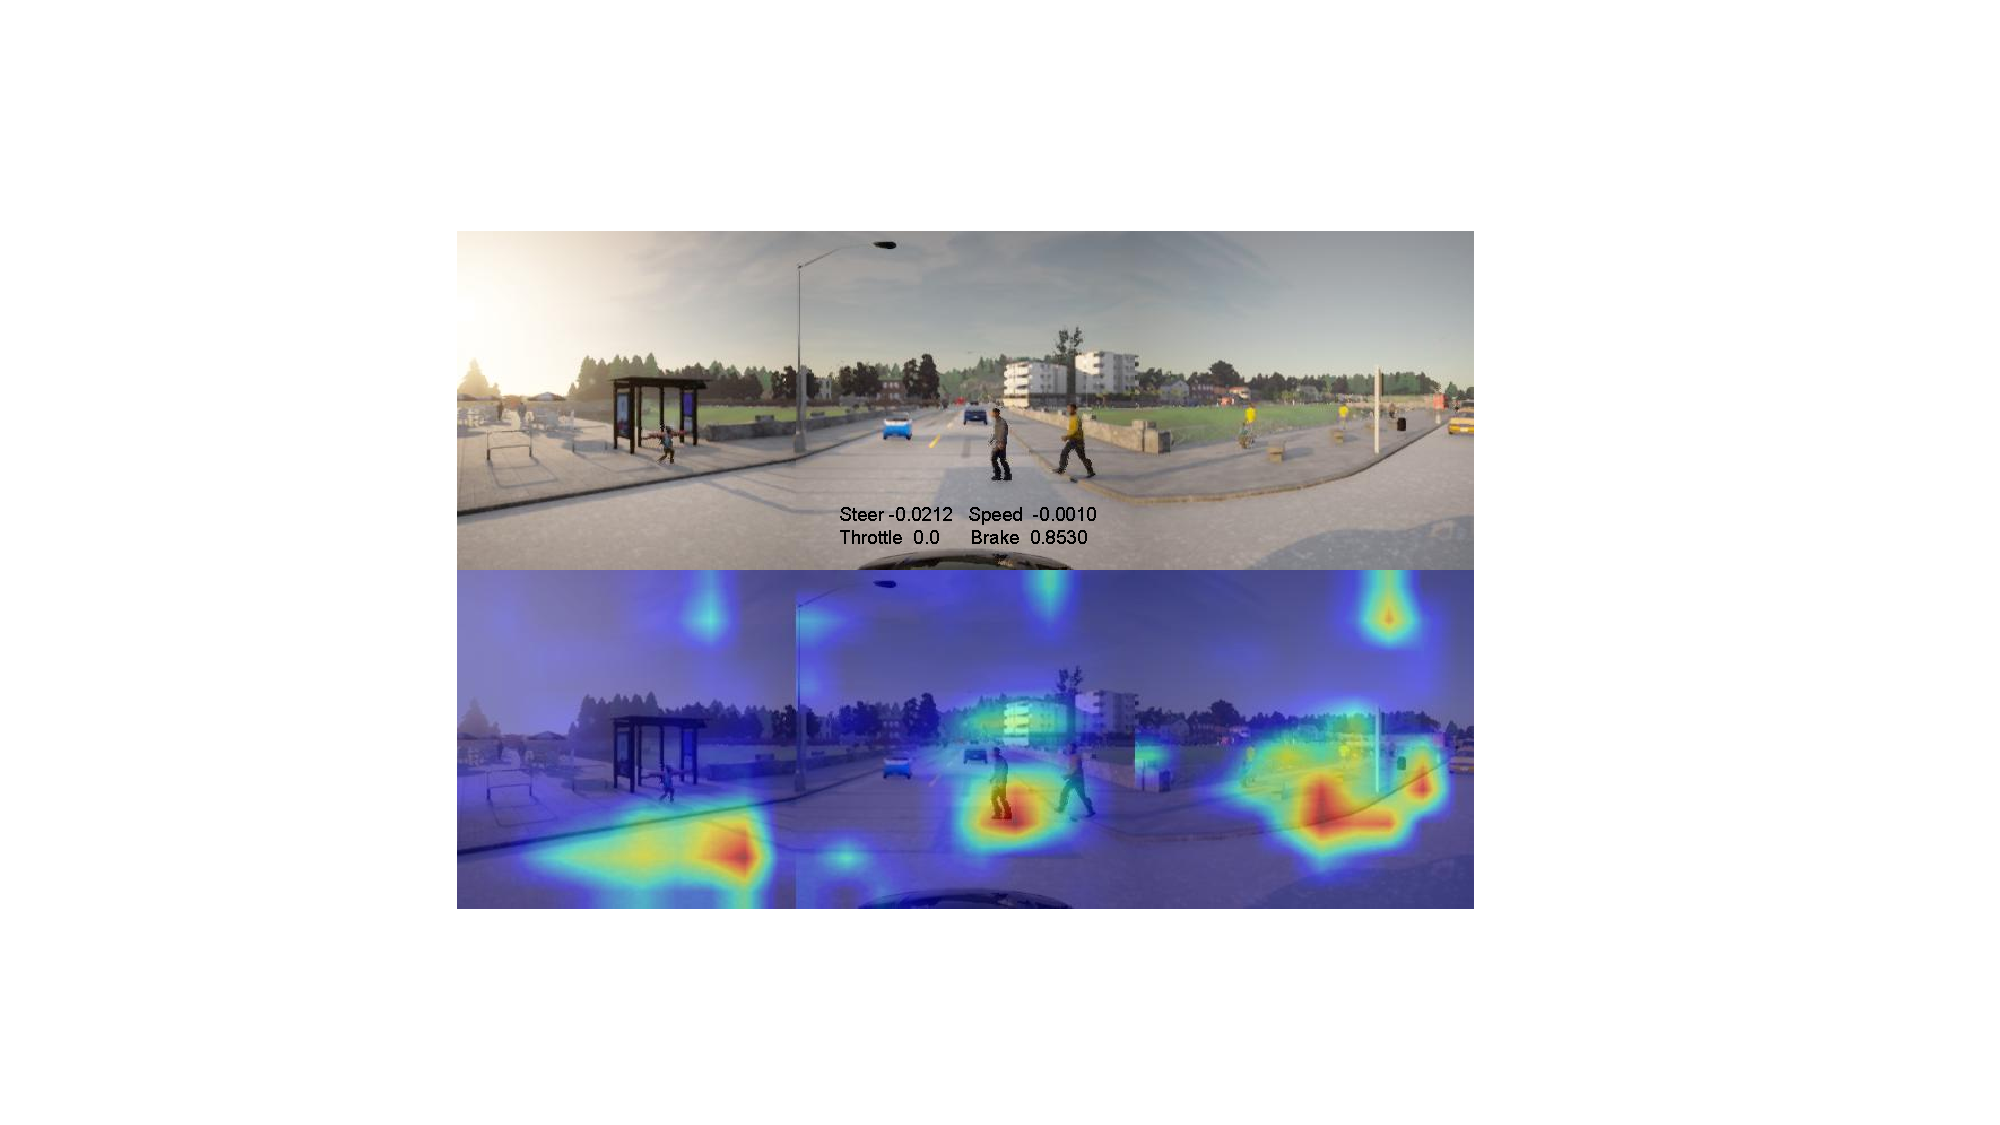
\includegraphics[width=\linewidth]{fig/attention_ped_greed.pdf}
%	\caption{Activation maps of BID at an intersection in Town02 show three highly activated image areas from driving viewpoints: 
%		the lane shoulder in the right, the crossing pedestrians in the center, and the driving area in the left. 
%		The causality between observation and action is demonstrated by a strong braking response (0.8530) due to the presence of pedestrians, despite the ``go-straight" command. 
%		This highlights BID's ability to prioritize pedestrian safety over other factors in BID's decision-making process. }
%	\label{fig:attention_ped_greed}
%\end{figure}



% 消融实验:速度(包括背侧通路)、导航
\subsubsection{Ablation}

\hspace{1pc}An imitation learning ego-vehicle's ability to perform is inherently constrained by the quality of experienced driver it imitates. 
Comparing imitation learning ego-vehicle trained on an experienced driver is pointless if that driver performs poorly.
This issue becomes apparent in a scenario never seen it before with crowded actors, where the performance of autopilot typically is poor. 
We optimize the BID (Fig.~\ref{fig:score_eu_lb_tt_tn}) and conduct ablation studies with architecture analysis (Fig.~\ref{fig:structure_analysis} and the crowded actors configuration (Table~\ref{table:infraction}) to establish a high precision effect and ensure a effective evaluation, allowing the proposed agent to attain a \emph{DS} of 96\%. 
As shown in Table~\ref{table:sucess_rate_nc_dense}, the optimal configuration from the ablative experiments is also assessed on benchmark in crowded actors for a more meaningful comparison with latest models.


% 说明消融的各个指标?
% L_N 导航信号
% L_D 背侧流信号
Fig.~\ref{fig:score_eu_lb_tt_tn} shows the behavior grades of experienced and imitation learning drivers for an epoch on offical benchmark with crowded actors.
The basic $\mathcal{L}$ represents the proposed implementation of the baseline BID trained by expert. 
According to the leaderboard instructions, this additional navigation vector helps separating scenes where the map's complexity may make it difficult to understand the labels of each frame.
Given the improvements in our best-performing BID, it is expected that $\mathcal{L}_D$ and $\mathcal{L}_D + \mathcal{L}_N$ gain better \emph{SR} than results described in Table~\ref{table:sucess_rate_nc_dense}.
The significant performance gap between the baseline and $\mathcal{L}_D + \mathcal{L}_N$, especially when transferring to the scene never seen it before, highlights the basic approach limitations.


% 一步步添加后的效果
$\mathcal{L}_D$ outperforms $\mathcal{L}_b$ overall by incorporating the dorsal stream and speed embedding into the baseline $\mathcal{L}_b$.
Additionally, learning from the action distribution allows $\mathcal{L}_D$ to generalize superior than $\mathcal{L}_b$ on the benchmark dataset, but not on the offical leaderboard.
When $E_S$ is given merely, the feature required to generate accurate driving action does representation mapping to enhance performance.
Since the expected path is given throught nagivation command in this instance, $E_N$ includes goal instructions.
The use of $E_N$ improves accuray for the benchmark because it encodes goal instruction, including the feature pointing to the following expected path.
To evaluate this idea, we utilize a integrated model structure in which the goal instruction described as one hot encoding is added to the evaluation feature $E_N$.
In the benchmark scene transferability evaluation, $\mathcal{L}_\text{BID}$ achieves the highest behavior degree in imitation learning ego-vehicles.



%
Adding supervised representation alongside feature matching accelerates the convergence of the process, as demonstrated by $\mathcal{L}_D + \mathcal{L}_N$.
However, when feature matching is omitted, supervised representation doesn't lead to better result with $\mathcal{L}_D$.
These suggests the possibility of value estimation and representation mapping working in tandem.
Predicting the value should be made easier by imitating the representation of RL-coach, which intuitively contains the feature needed for value prediction. 
In turn, these estimation can be enhanced by regularizing representation mapping, improving overall performance.


\subsubsection{Infraction and Result Analysis}


\hspace{1pc}Table~\ref{table:infraction} presents a particular result and infraction analyse on the benchmark dataset with crowded actors in the scene never seen it before. 
Interestingly, the remarkably better \emph{ABD} degree in the basic $\mathcal{L}_b)$ is primarily caused by results from heavy rains. 
The issue is significantly reduced by imitating expert leading to a 23\% absolute improvement in the \emph{DS} for $\mathcal{L}_D$.
While maintaining the same IL strategy, this gain illustrates the advantages of using a more knowledgeable driver. 
Better improvements are achieved with the addition of soft targets and latent feature supervision in $\mathcal{L}_D+\mathcal{L}_N$, resulting in another 30\% absolute increase in performance. 
By handling red lights more effectively, this BID agent achieves a driving score of 89\%, reaching expert-level performance with just camera image as input.





 
\section{Discussion and conclusion}
\label{sec:conclusion}
\hspace{1pc}This paper has presented a novel neuro-inspired mapping system with 4 degrees of freedom for 3D environments known as NeuroSLAM.
In this system, we modeled the 3D grid cells and the multilayered head direction cells representing the robot's 4DoF pose in 3D environments.
Similar to the mamalian vision perception capability, the system is noly coupled with a lightweight vision system that provides external visual cues and self-motion cues.
The system built multilayered experience maps with synthetic and real-world datasets consisting by indoor and outdoor parts.
The relocalization and loop closure are driven by the multilayered experience map through sequences of familiar visual cues.
The experimental results demonstrated the system's capability to generate coherent 3D experience maps with consistent topology in simulated and real-world 3D environments, and to process loop closure with significant errors in path integration.


The conjunctive pose cell model combines both 3D grid cells and head direction cells, enabling it to represent a robot's 4DoF pose at an arbitrary 3D location in 3D environments.
It is distinctive from the RatSLAM model which uses pose cells to represent 2D pose $ (x, y, \theta) $.
We modeled the 3D grid cells and multilayered head direction cell respectively rather than using a type of combined cell model.
Our conjunctive pose cell model can represent a robot's pose when moving through horizontal and vertical space.
Comparing with other research (see section 2.2), our model is distinctive and can represent 4DoF pose in 3D space.
To the best of our knowledge, the novel discovery of head direction cells and 3D grid cells have not been modeled for 3D SLAM so far.
The NeuroSLAM systems has some explorary value in investigating how 5DoF or 6DoF biologically-plausible SLAM systems could be implemented.


In mammals, the functional relationship between head directions cells and 3D grid cells is still not entirely clear.
In our model, we modeled these two types of cells separately.
But a speculative connection between 3D grid cells and head direction cells was also proposed.
The system processed the path integration in a 3D grid cell network using the direction information decoded from the multilayered head direction cell network.
In order to improve computing efficiency and reduce the complexity of the system, we simplified the neural model.
We don't build the 3D place cell model.
However, we represent the functional properties of place cells in the 3D grid cell netwrok and the 3D experience map.
This model may be helpful to neuroscientists in suggesting experiments for interpreting the neural mechanisms of 3D spatial representation supported by head direction cells and 3D grid cells.
As shown in the experimental results of 3D grid cells activity and multilayered head direction cells activity, the trajectory of active cells in the 3D grid cell network has similar characters of a regular 3D lattice pattern compared with the 3D FCC model.
The simplified model of multilayered head direction cells worked well enough for representing 4DoF pose in 3D environment though we didn't take incorporate the 3D head direction cells found in mammals into consideration.
The 3D head direction cells respond to a particular combination of azimuth x pitch thus representing the direction of the head vector in 3D space.
Finkelstein et al. proposed a toroidal model for modeling 3D head direction cells.
The model can only represent yaw and pitch.
We are looking to expand our model to represent 6DoF pose with complex 3D head direction cells, e.g. a 3D cube head direction network or conjunctive 3D head direction cell network consisting of a toroidal network and a ring network in future work.


NeuroSLAM has some advantages over the conventional SLAM methods from the perspective of 3D space encoding, 3D path integration, 3D pose representation, and the performance.
Firstly, we encode the experience map with the conjunctive code of 3D grid cells, head direction cells, and local view cells, which not only can encode experience robustly but also can keep biological plausibility.
This encoding method can also reduce false positives and repeately correct loop closure even facing accumulative odometry error.
When matching familiar places, we use both the threshold of scene similarity and the distance threshold of conjunctive codes of experiences.
In contrast, the conventional methods encode places only by geometric coordinates and implement familiar place recognition only based on feature matching which are not robust in featureless or dynamic environments particularly.
Furthermore, NeuroSLAM can reuse existed experiences and add little new experiences when revisiting familiar scenes like humans do.
However, the conventional methods, e.g. ORB-SLAM and LDSO, generate a lot of pose nodes continuously along trajectories which increases the computational complexity and power cosumption in large environments.
% 航迹推算
Secondly, the 3D state estimation by path integration (dead reckoning) is also one of key modules in SLAM systems.
The conventional SLAM methods are often implemented based on filters or optimization, e.g. ORB-SLAM and LDSO, which assume that the functions of state transition and measurement are linear and the noises and Gaussian noises.
The performance of the SLAM system based on optimization or based on the Filters, e.g. Kalman Filter, extended Kalman Filter and Particle Filter, also suffers when increasing the number of landmarks.
All previous landmark estimations are affected with every new added landmark.
This can be difficult or even infeasible for long term task in large complex environments, where the robot faces a huge amount of landmarks.
Due to these restrictions, these methods can not capable of performing mapping in real-time, unpredictable environments.
However, the NeuroSLAM system could enable robots to locate and map their surrounding environments robustly compared to the conventional SLAM methods, since the 3D grid cell model based on the attractor neural network is capable of processing non-linear state estimation by path integration using neural dynamics in extreme unpredictable environments, e.g., light or scenes change, quick motion change.
The neural dynamics of excitation and inhibition is able to estimate the robot's pose state by combining self-motion and local view cues reliably.
Thirdly, NeuroSLAM represents a balance between limited 2D RatSLAM type implementations and full 6DoF implementations like ORB-SLAM, NeuroSLAM is in the middle, and exploits constraints that are reasonable (e.g. no roll) for a range of applications that ORB-SLAM doesnt.
Finally, the NeuroSLAM model can potentially be built based on brain-inspired neuromorphic chip with advantages of low power consumption, high computational efficiency in future work.
NeuroSLAMs origins in biological inspiration means that it also has the potential to incorporate further discoveries and mechanisms as they are discovered in the mammalian brain.
For instance, we can integrate the NeuroSLAM system with an episodic memory module to improve the adaptivity in unpredictable environments like human do.
Overall, these properties enable NeuroSLAM to have competitive performance with conventional methods.
The brain-inspired methods show the potential to push SLAM to a new level in large, unstructured, unpredictable environments.


Although we use a lightweight visual odometry system here that is only capable of generating relatively coarse estimates of motion with 4 degrees of greedom, there is the potential to integrate this model with a full 6DoF visual odometry system from the conventional robotics literature such as LIBVISO2 and a multitude of other equivalent techniques.
While this may reduce the biological relevance of the results, it will also increase the metric accuracy of the experience maps generated by NeuroSLAM, making it more useful for applications where metric accuracy, especially global metric accuracy, is critical.
Likewise, future work could improve loop closure robustness to varying environmental conditions and camera viewpoints by incorporating a mroe sophisticated visual place recognition process, for example utilizing semantics and state-of-the-art learnt features.


The 3D multilayered experience map generated by the NeuroSLAM system can be learned and generated when the robot visits unknown environments.
It can also be maintained and updated based on the learning and recalling mechanism incrementally.
The 3D spatial experience nodes represent 4DoF pose in specific 3D location, and the links contain distance and direction between nodes.
This metric and topology information can be used for 3D path planning and guidance control in 3D environments.
It's likely that map maintenance routines, as implemented in prior work could also be deployed here to ensure long-term map stability as well as computation and storage visbility.
We are looking to test the utility of these experience maps for real robot navigation in future work.
























%\section*{Acknowledgments}
%The authors gratefully acknowledge the financial support provided by the Natural Science Foundation of Hunan Province (No.2024JJ6190), the Open Project of Xiangjiang Laboratory (No.23XJ03009), Xiangjiang Laboratory major program subproject (No.22XJ01001-2), the "Digital Intelligence +" interdisciplinary research project of Hunan University Of Technology and Business (No.2023SZJ19), Scientific research project of Hunan Provincial Department of Education (No.22B0646), Research on a new generation of brain-like intelligent computing framework based on ultra-large-scale real neural systems (24XJJCYJ01001).


\bibliography{BID.bib}
% 指定风格必不可少,否则参考文献都是问号
\bibliographystyle{IEEEtran}


\newpage
% 作者信息
\begin{IEEEbiography}[{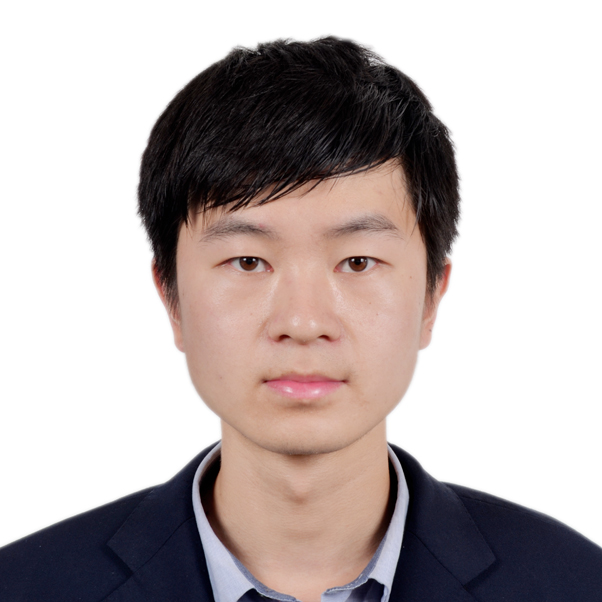
\includegraphics[width=1in,height=1.25in,clip,keepaspectratio]{./fig/HaidongWang}}]{Haidong Wang}
	 received the B.E. degree in Computer Science and Technology from Hunan University Of Technology and Business, the M.Sc. degree in Computer Technology from the University of Chinese Academy of Sciences (UCAS), Beijing, China, in 2017, and the Ph.D. degree in Computer Science and Technology from Hunan University, Changsha, China, in 2022. Since 2022, he joined Hunan University Of Technology and Business. His current research interests include bran-like perception, autonomous driving and reinforcement learning.
\end{IEEEbiography}

% 作者信息
\begin{IEEEbiography}[{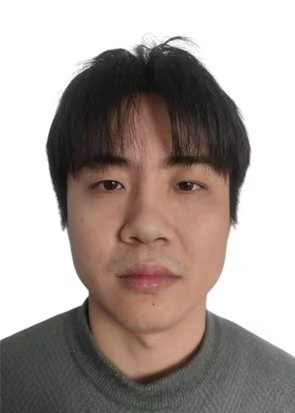
\includegraphics[width=1in,height=1.25in,clip,keepaspectratio]{./fig/PengfeiXiao}}]{Pengfei Xiao}
	is currently pursuing the M.Sc. degree in Computer Science and Technology from Hunan University Of Technology and Business, Changsha, China. He has a deep understanding of theoretical knowledge and tools related to brain-like computing, and has engineering experience in autonomous driving, traffic simulation. His current research interests include machine learning, multi-object tracking and reinforcement learning.
\end{IEEEbiography}

\vfill

\end{document}


